\chapter{Performance Analysis}
\label{cha:pa}

The purpose of this chapter is to examine and discuss the project's performance
impact both on execution time and on memory usage. Firstly, we present the
execution time overhead between a standard binary and a protected one. During this
analysis we give great importance to the time overhead, describing the meaning
of the collected data. Secondly, we present the memory footprint of the Control
Flow Integrity enforcer. Lastly, we provide an analysis of the obtained results
as well as some optimization ideas to further reduce the performance impact on
the code.

The performance analysis took inspiration from the articles \textit{Efficient
CFI Enforcement for Embedded Systems Using ARM TrustZone-M} (Gisu Yeo, Yeryeong Kim
et al., 2022)\cite{article1} and \textit{PROLEPSIS: Binary Analysis and Instrumentation
of IoT Software for Control-Flow Integrity} (Valentina Forte, Nicol\`{o} Maunero
et al., 2021)\cite{article2} where the writers propose similar solutions to
enforce Control Flow Integrity on \textit{ARM}-based embedded devices. We tested
the infrastructure on the same algorithms proposed by the papers, providing tests
on $13$ different algorithms + $4$ variations with ``forced'' indirect jumps\footnote{Indirect
jumps were ``forced'' using volatile function pointers of the \textit{C} programming
language.}.

Note that, to present correct and realistic data, all tests have been conducted
on the aforementioned \textit{Espressif's ESP32-C3-DevKitM-1}.

\section{Time Overhead}
\label{sec:pa_time}

In this section, we discuss how the infrastructure affects the execution time of
the code. Two histograms depicting test results can be seen in Figures
\ref{fig:lowtime} and \ref{fig:hightime}, note that execution times have been separated
into two different charts to enhance readability of data.

\begin{figure}[htbp]
  \centering
  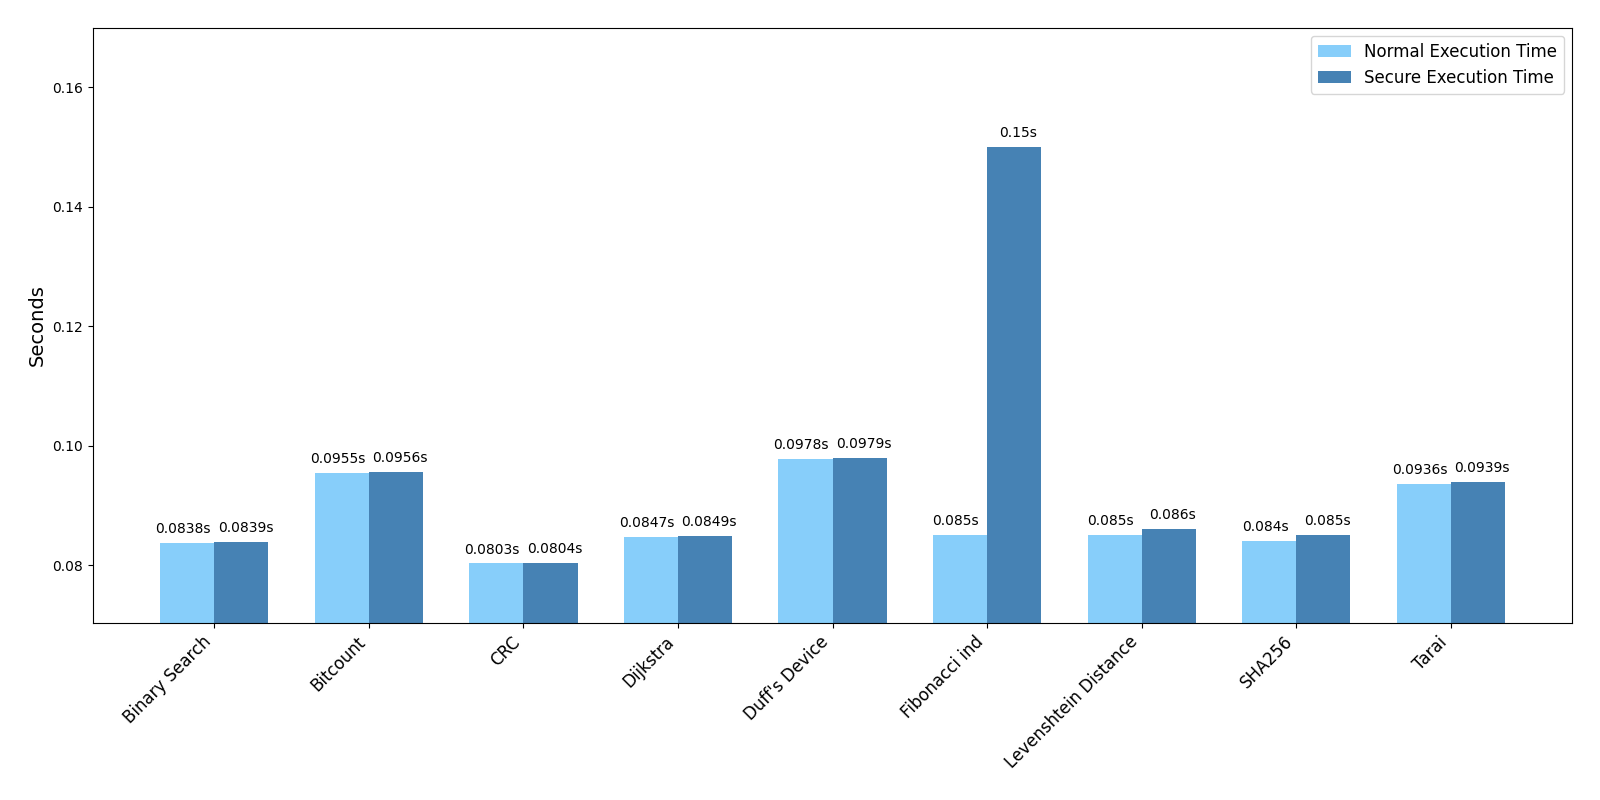
\includegraphics[width=\linewidth]{images/low_times.png}
  \caption{Comparison between binaries execution times (low times)}
  \label{fig:lowtime}
\end{figure}

\begin{figure}[htbp]
  \centering
  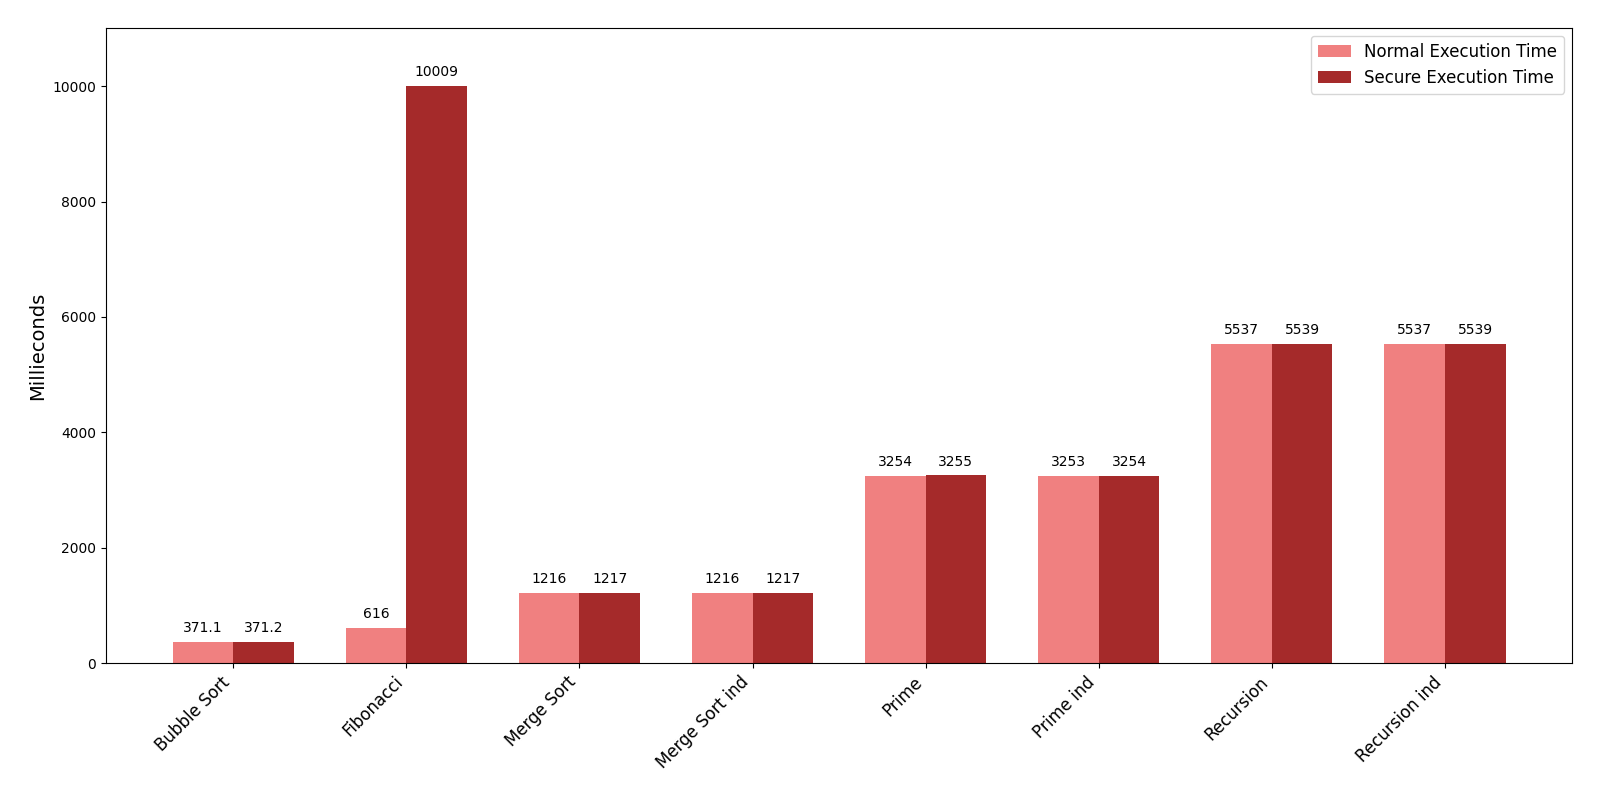
\includegraphics[width=\linewidth]{images/high_times.png}
  \caption{Comparison between binaries execution times (medium and high times)}
  \label{fig:hightime}
\end{figure}

Table \ref{tab:times} depicts test results for each algorithm as well as the percentage
of time overhead. In most cases the time increases by few milliseconds or less, resulting
in an unnoticeable increase in execution time. However, there are two cases in which
the time overhead is big and it impacts performances in a relevant way.

\begin{table}
  \centering
  \begin{tabular}{|c|c|c|c|}
    \hline
    \textbf{Algorithm}                   & \textbf{Normal run time (ms)} & \textbf{Secure run time (ms)} & \textbf{Time Overhead} \\
    \hhline{====} \textit{Binary Search} & $83.87$                       & $83.88$                       & $0.012\%$              \\
    \hline
    \textit{Bitcount}                    & $95.5$                        & $95.6$                        & $0.11\%$               \\
    \hline
    \textit{Bubble Sort}                 & $371.13$                      & $371.16$                      & $0.008\%$              \\
    \hline
    \textit{CRC}                         & $80.25$                       & $80.26$                       & $0.012\%$              \\
    \hline
    \textit{Dijkstra}                    & $84.7$                        & $84.9$                        & $0.236\%$              \\
    \hline
    \textit{Duff's Device}               & $97.795$                      & $97.799$                      & $0.0041\%$             \\
    \hline
    \textit{Fibonacci}                   & $616.6$                       & $10008.9$                     & $1523.24\%$            \\
    \hline
    \textit{Fibonacci Indirect}          & $84.9$                        & $151.1$                       & $77.97\%$              \\
    \hline
    \textit{Levenshtein Distance}        & $85$                          & $86$                          & $1.176\%$              \\
    \hline
    \textit{Merge Sort}                  & $1216$                        & $1217$                        & $0.0822\%$             \\
    \hline
    \textit{Merge Sort Indirect}         & $1216.8$                      & $1216.9$                      & $0.0082\%$             \\
    \hline
    \textit{Prime}                       & $3254$                        & $3255$                        & $0.03\%$               \\
    \hline
    \textit{Prime Indirect}              & $3253$                        & $3254$                        & $0.03\%$               \\
    \hline
    \textit{Recursion}                   & $5537$                        & $5539$                        & $0.036\%$              \\
    \hline
    \textit{Recursion Indirect}          & $5537$                        & $5539$                        & $0.036\%$              \\
    \hline
    \textit{SHA256}                      & $84$                          & $85$                          & $1.19\%$               \\
    \hline
    \textit{Tarai}                       & $93.6$                        & $93.9$                        & $0.32\%$               \\
    \hline
  \end{tabular}
  \caption{Test results for execution times}
  \label{tab:times}
\end{table}

It is straightforward to understand why the overhead is small for algorithms
like \textit{Binary Search} or \textit{Duff's Device} since these programs
perform few jump instructions and most of the computation is performed inside a
while or for loop so, the overhead given by the instrumentation is unnoticeable if
compared to the total execution time. For example, the \textit{Binary Search}
algorithm performs $3$ jump instruction and $3$ return instructions even if it
is working on a rather big input array. This means that, despite the size of the
input, the Control Flow Integrity enforcer is called only $6$ times, resulting
in a small time overhead. We want to specify that this behavior is expected in these
situations.

Instead, examples like \textit{Prime} and \textit{Recursive} are a bit trickier.
Since these algorithms work with a recursive approach they perform many control transfer
instructions consequently thus, we expect the time required for the context
switch and the forward and backward edge controls to be somewhat impactful. However,
results show that even in these cases the difference is barely noticeable\footnote{In
these cases instead of increasing the execution time by less then a millisecond,
we see an increase of few milliseconds.}. The reason could be due to the
processor's frequency which, in the case of \textit{Espressif's ESP32-C3-DevKitM-1},
is $160 \ MHz$. This means that the CPU is able to execute the secure and non-secure
binaries in similar times. For example, the \textit{Recursion} algorithm performs
$\sim 4000$ jump instructions and $\sim 4000$ return instructions which translates
to $\sim 8000$ edge controls and $\sim 16000$ context switches\footnote{The
number is doubled because for each edge control we need to increase the
privilege to M-mode, perform the control, and then return to U-mode, resulting in
two context switches.}. However, if we compare those numbers to the $160$
million operations the processor can perform in a second we see why the time
overhead is so small. Note that we add $2$ instructions for every jump instruction
and $3$ instructions for every return instruction, resulting in an instruction
overhead of $4000*2 + 4000*3 = 20000$. Moreover, the handling of forward and
backward edge controls requires $\sim 180$ instructions which results in
$(4000 + 4000) * 180 = 1440000$ total instructions. Resulting in a total instruction
overhead of $20000 + 1440000 \simeq 1460000$ instructions. Now, if we compute $\frac{1460000}{160000000}$
we discover that the utilized processor can perform all these instructions in $\sim
9.125$ milliseconds. Depending on the algorithm and the recursion depth we see
that the overhead is affecting the execution time by few milliseconds.

Two peculiar cases are the ones of the \textit{Fibonacci} and \textit{Fibonacci
Indirect} algorithms, in these cases, the overheads are $1523.24\%$ and
$77.97\%$ respectively. The possible reason for these enormous overheads is that
these algorithms make two recursive calls each time so we end up with an exponential
amount of jump and return instructions. This leads to many invocations of the
Control Flow Integrity enforcer and the execution time is strongly affected by
this.

Overall, we achieved an average time overhead of $94.38\%$ with a standard deviation
of $368.68$. However, if we do not take into account the outliers we can see that
the median is $0.036\%$. These results clearly show that the time overhead is
almost unnoticeable in many cases but, this also demonstrates that the project strongly
suffers from deeply recursive algorithms and that further optimization is required
to reduce the time impact on these types of algorithms.

Lastly, in Table \ref{tab:othertimes} we provide the times required to
instrument the code, extract the Control Flow Graph, and perform the simulation.
The instrumentation and CFG extraction phases always require less than a fraction
of a second to finish. However, we must take into consideration that the tested algorithms
are composed of few lines of code and the situation could change if we were to instrument
a firmware composed of thousands of lines. The simulation instead requires a lot
of time, even algorithms that run in a second or less require some seconds to simulate.
This is due to the logging required to extract the indirect jump destinations
which affects the time performances seriously. Note that we can accept this result
since the simulation is run only once and the logging is removed from the final binary
so that this overhead does not affect the actual execution time.

\begin{table}
  \centering
  \begin{tabular}{|c|c|c|c|}
    \hline
    \textbf{Algorithm}                   & \textbf{Instrumentation (ms)} & \textbf{Simulation (ms)} & \textbf{CFG extraction (ms)} \\
    \hhline{====} \textit{Binary Search} & $2.96$                        & no simulation            & $1.74$                       \\
    \hline
    \textit{Bitcount}                    & $1.96$                        & no simulation            & $1.53$                       \\
    \hline
    \textit{Bubble Sort}                 & $3.02$                        & no simulation            & $1.75$                       \\
    \hline
    \textit{CRC}                         & $2.03$                        & no simulation            & $1.54$                       \\
    \hline
    \textit{Dijkstra}                    & $2.64$                        & no simulation            & $1.82$                       \\
    \hline
    \textit{Duff's Device}               & $2.65$                        & no simulation            & $1.63$                       \\
    \hline
    \textit{Fibonacci}                   & $2.09$                        & no simulation            & $1.49$                       \\
    \hline
    \textit{Fibonacci Indirect}          & $2.02$                        & $130556.7$               & $70.37$                      \\
    \hline
    \textit{Levenshtein Distance}        & $2.55$                        & no simulation            & $1.67$                       \\
    \hline
    \textit{Merge Sort}                  & $3.54$                        & no simulation            & $1.78$                       \\
    \hline
    \textit{Merge Sort Indirect}         & $3.6$                         & $4639.4$                 & $2.73$                       \\
    \hline
    \textit{Prime}                       & $2.14$                        & no simulation            & $1.68$                       \\
    \hline
    \textit{Prime Indirect}              & $2.08$                        & $11405.1$                & $4.51$                       \\
    \hline
    \textit{Recursion}                   & $2.02$                        & no simulation            & $1.59$                       \\
    \hline
    \textit{Recursion Indirect}          & $2.02$                        & $23275.1$                & $8.75$                       \\
    \hline
    \textit{SHA256}                      & $4.11$                        & no simulation            & $1.89$                       \\
    \hline
    \textit{Tarai}                       & $1.98$                        & no simulation            & $1.52$                       \\
    \hline
  \end{tabular}
  \caption{Test results for instrumentation, simulation, and CFG extraction
  phases}
  \label{tab:othertimes}
\end{table}

\section{Memory Overhead}
\label{sec:pa_memory}

In this section, we showcase how the infrastructure affects the size of the
produced binary. A histogram depicting test results can be seen in Figure \ref{fig:binsize}.

\begin{figure}[htbp]
  \centering
  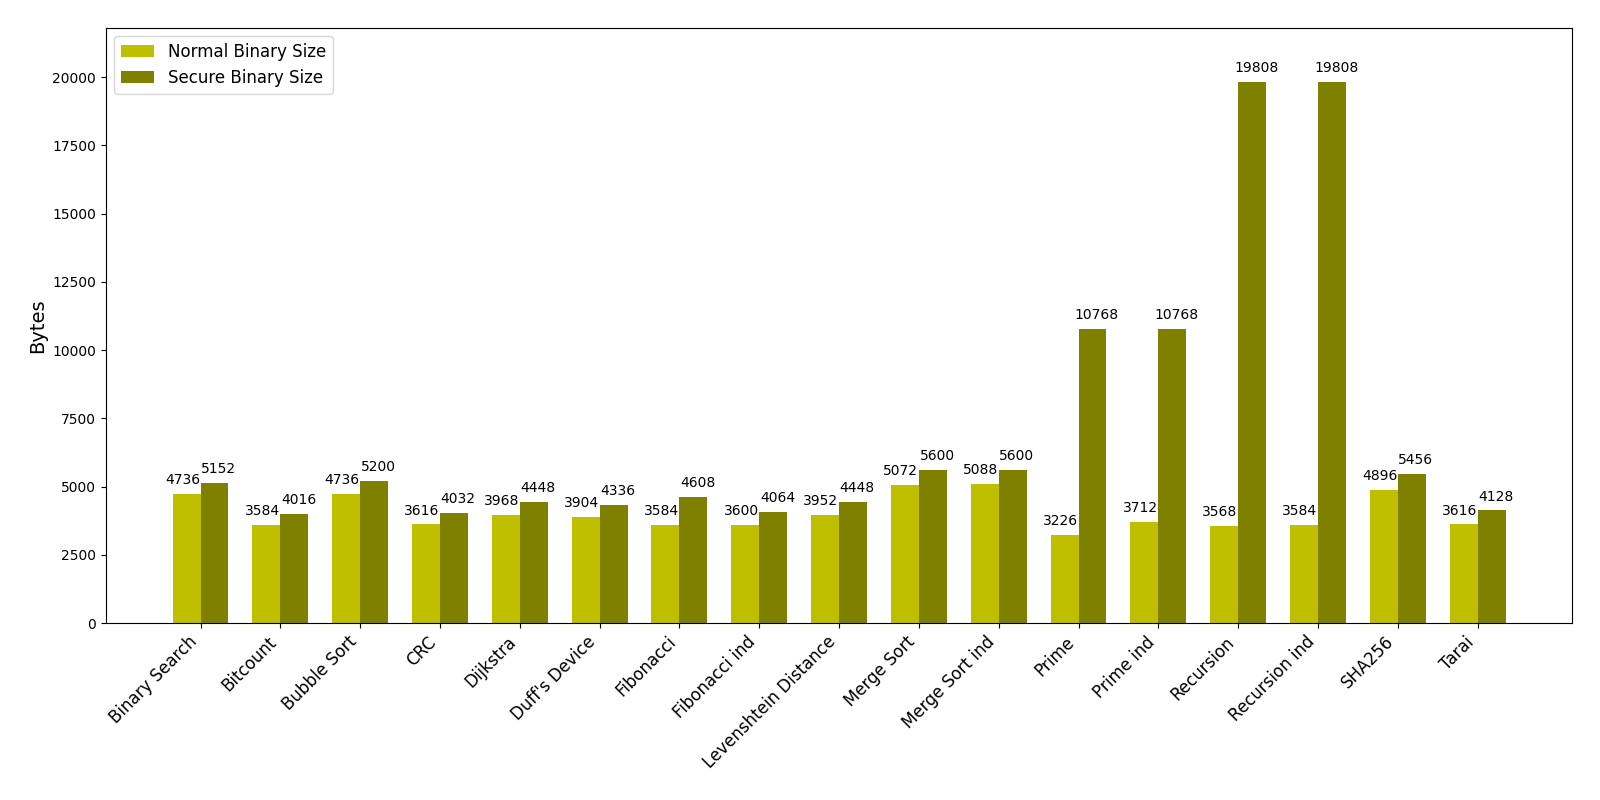
\includegraphics[width=\linewidth]{images/size.png}
  \caption{Comparison between binaries size}
  \label{fig:binsize}
\end{figure}

Table \ref{tab:binsize} depicts test results for each algorithm as well as the
percentage of memory overhead. As we can see, in most cases the size of the
binary increases by $\sim 10\%$. This is due to the shadow stack, Control Flow
Graph, and the instructions added during instrumentation.

As for the time overhead analysis, there are some peculiar cases. \textit{Prime},
\textit{Recursion} and their indirect variations \textit{Prime Indirect} and \textit{Recursion
Indirect}, present a memory overhead of $\sim 200\%$ and $\sim 450\%$ respectively.
This happens because these recursive algorithms perform all the jump
instructions consecutively and then all the return instructions. This means that
we must allocate a shadow stack big enough to store all the return addresses to ensure
correct backward edge controls. For example, we have seen that the \textit{Recursion}
algorithm performs $\sim 4000$ jump instructions, this means that we must create
a shadow stack able to store at least $4000$ addresses. Given that an address is
stored as an \textit{unsigned int}, we can easily see that a shadow stack that
can store $4000$ addresses occupies $4000*4 = 16000 \ \textit{Bytes}$\footnote{We
multiply by $4$ because it is the size of an \textit{unsigned int} in C.}. Now, if
we take the size of the secure binary for the \textit{Recursion} algorithm we
can calculate $19808 - 16000 = 3808 \ \textit{Bytes}$, so, apart from the shadow
stack, the binary has a memory overhead of $\frac{3808-3568}{3568}*100 = \sim 6.
73\%$ which is similar to other ones.

Note that this problem is related strictly to recursive algorithms as they perform
a high number of jumps and then they start performing the first return instruction.
However, we could have a similar problem with the Control Flow Graph as for a big
binary like a firmware we can have many different jump instructions, and, as a consequence,
the CFG would drastically increase in size.

\begin{table}
  \centering
  \begin{tabular}{|c|c|c|c|}
    \hline
    \textbf{Algorithm}                   & \textbf{Normal bin size (B)} & \textbf{Secure bin size (B)} & \textbf{Memory Overhead} \\
    \hhline{====} \textit{Binary Search} & 4736                         & 5152                         & $8.78\%$                 \\
    \hline
    \textit{Bitcount}                    & 3584                         & 4016                         & $12.05\%$                \\
    \hline
    \textit{Bubble Sort}                 & 4736                         & 5200                         & $9.79\%$                 \\
    \hline
    \textit{CRC}                         & 3616                         & 4032                         & $11.51\%$                \\
    \hline
    \textit{Dijkstra}                    & 3968                         & 4448                         & $12.09\%$                \\
    \hline
    \textit{Duff's Device}               & 3904                         & 4336                         & $11.06\%$                \\
    \hline
    \textit{Fibonacci}                   & 3584                         & 4608                         & $28.57\%$                \\
    \hline
    \textit{Fibonacci Indirect}          & 3600                         & 4064                         & $12.88\%$                \\
    \hline
    \textit{Levenshtein Distance}        & 3952                         & 4448                         & $12.55\%$                \\
    \hline
    \textit{Merge Sort}                  & 5072                         & 5600                         & $10.41\%$                \\
    \hline
    \textit{Merge Sort Indirect}         & 5088                         & 5600                         & $10.06\%$                \\
    \hline
    \textit{Prime}                       & 3226                         & 10768                        & $233.78\%$               \\
    \hline
    \textit{Prime Indirect}              & 3712                         & 10768                        & $190.08\%$               \\
    \hline
    \textit{Recursion}                   & 3568                         & 19808                        & $455.15\%$               \\
    \hline
    \textit{Recursion Indirect}          & 3584                         & 19808                        & $452.68\%$               \\
    \hline
    \textit{SHA256}                      & 4896                         & 5456                         & $11.43\%$                \\
    \hline
    \textit{Tarai}                       & 3616                         & 4128                         & $14.16\%$                \\
    \hline
  \end{tabular}
  \caption{Test results for memory consumption}
  \label{tab:binsize}
\end{table}

Overall, we achieved an average memory overhead of $88.06\%$ with a standard
deviation of $152.77$. However, similarly to the time overhead, if we do not take
into consideration the outliers we can see that the median is $12.09 \%$. These
results show that in most cases the project can produce a secure binary without
affecting too much memory consumption. Even in this case, the project suffers
from deeply recursive algorithms as we need to allocate a bigger shadow stack to
accommodate space for a secure storage of each return address.

\section{Results and Analysis}
\label{sec:pa_results}

In this section, we discuss the obtained result and showcase the weak points of
the implementation.

As we have seen in the previous sections the project showcases promising
performances in most cases. In almost all the tested algorithms time overhead was
barely noticeable and memory consumption was acceptable. Overall, the project infrastructure
is not impacting the performances of the executable.

However, in the case of deeply recursive algorithms, we have seen that the time overhead
grows exponentially due to the high number of control transfer instructions and the
related forward and backward edge controls. Also, the size of the binary grows as
we need a bigger shadow stack to store all the addresses needed to perform the backward
edge controls.

Moreover, we have seen that if the code is composed of thousands of lines it is
likely that the Control Flow Graph will be very big. This is because if we have many
jump instructions from different sources to different destinations we must store
each pair, thus the space occupied by the CFG grows.

Similar results have been obtained in the already cited paper \textit{PROLEPSIS:
Binary Analysis and Instrumentation of IoT Software for Control-Flow Integrity}\cite{article2}
where the writers introduced an average instruction overhead of $\sim 4\%$. Unfortunately,
given the fact that the writers proposed a preliminary prototype they do not
provide the execution time overhead introduced with their technology. Moreover,
the paper \textit{Efficient CFI Enforcement for Embedded Systems Using ARM
TrustZone-M}\cite{article1} presents an average execution time overhead of
$159.3 \%$, with the lowest overhead being $0.2 \%$ and the highest being $652.27
\%$. Additionally, the writers say that they saw an average $7.36\%$ increase in
memory consumption. With this results we can effectively say that the proposed
solution to enforce Control Flow Integrity achieved standard overheads in both
execution time and memory consumption, making it a valuable choice for embedded systems.

In the following section, we provide some optimization techniques that could be
applied to further increase the performances. Specifically, we provide
alternative solutions to improve the weak points of the project.

\section{Optimization Techniques}
\label{sec:pa_optimization}

Since optimization is a key factor when developing projects on embedded devices given
their hardware limitations we tried to provide an infrastructure as fast as possible
while preserving memory usage. However, as test results show, there are some
aspects of the project that require further improvement to be considered
acceptable.

The two identified cases in which the project strongly impacts the performances
are:
\begin{itemize}
  \item Deeply recursive algorithms: we have seen that deeply recursive
    algorithms require a big shadow stack to hold all the return addresses and
    thus, they require a lot of extra memory. To solve this issue we could
    modify the shadow stack in the following way. When we see that a function calls
    itself many times we could store the return address only one time and introduce
    a \textit{peek} function. With this, we could still perform the backward
    edge controls when we need to but we would need to store the address only
    once. Then, if we need to perform a control on another address we would just
    need to \textit{pop} the ``recursive'' address and then \textit{pop} the
    following one to see if it matches with the one we are checking. With such modification,
    we could effectively reduce the amount of space occupied by the shadow stack
    in case of recursive algorithms without impacting the provided security
    features;

  \item Big user code: we have seen that with very a big codebase (like the aforementioned
    firmware one) we could end up in a situation where the Control Flow Graph
    grows bigger and bigger due to the high amount of control transfer
    instructions from different sources to different destinations. Unfortunately,
    we can do nothing about memory consumption in this case as we can't afford
    to avoid storing some source-destination pairs. However, as already
    explained we could implement a Hash Table which would not decrease the
    memory consumption but, at least we could reduce the time required to access
    the Control Flow Graph from $\mathcal{O}(\log{n})$ to $\mathcal{O}(1)$;

  \item Small user code: lastly, we provide a space optimization solution that could
    be implemented for very small source code. Say, for example, that the
    \textit{.text} section that we want to instrument starts at address $0x4038A0
    00$ and ends at address $0x4038F000$. Since the first part of the address
    stays the same it provides no useful information, thus we could apply a bit-mask
    to remove $4038$ from the address, storing only the last $16$ bits. This means
    that we would be able to store an address as an \textit{unsigned short}
    instead of an \textit{unsigned int}. As a result, we would be able to halve the
    space required to store the Control Flow Graph and the shadow stack resulting
    in a great improvement in memory consumption. However, this solution only works
    when the user code is very small because if the \textit{.text} section
    starts at address $0x4038A000$ and ends at address $0x4039F000$ we would
    still need an \textit{unsigned int} to store a correct representation of the
    address.
\end{itemize}

In conclusion, this analysis has demonstrated that our project exhibits commendable
performance in a variety of scenarios. Nevertheless, there are specific edge cases
where its efficiency can be significantly compromised, leading to suboptimal
results. These instances reveal potential vulnerabilities in the system that could
hinder its overall effectiveness. To address these challenges, we suggest implementing
the proposed solutions, which aim to refine the project's functionality. By fine-tuning
the system to better adapt to particular situations, we can effectively minimize
both memory usage and execution time, thereby enhancing the overall performance and
reliability.
